\documentclass[oneside]{book}

% Load the VUB package.
% This has many options, please read the documentation at
% https://gitlab.com/rubdos/texlive-vub
\usepackage{vub}

%href package to make references clickable.
\usepackage{hyperref}
\hypersetup{
    colorlinks,
    citecolor=black,
    filecolor=black,
    linkcolor=black,
    urlcolor=black
}

% Some highly suggested packages, please read their manuals.
\usepackage{cleveref}
\usepackage[natbib,style=apa]{biblatex}
\addbibresource{../bibliography.bib}
\usepackage{listings}
\usepackage{wrapfig}

%space between paragraph and indent all
\setlength{\parskip}{1em}
\usepackage{indentfirst}

%space between bib entries
\setlength\bibitemsep{2\itemsep}

%images settings
\graphicspath{ {./images/} }
\usepackage{graphicx,caption}
\usepackage{float}
\usepackage{rotating}
\usepackage{tikz}

% subfigures
\usepackage{subcaption}

%fix section numbering for use with parts
\renewcommand*\thepart{\Roman{part}}
\makeatletter
\@addtoreset{section}{part}
\makeatother
\renewcommand*\thesection{\arabic{part}.\arabic{section}}
\renewcommand*\thesubsection{\thesection.\arabic{subsection}}

%START title
\title{Computer generated car design}
\subtitle{Assignment 1 - Computational Creativity}
\author{Lennert Bontinck}
\date{February, 2020-2021}
\promotors{Student number: 568702}
\faculty{Computer Science: AI}
\begin{document}
\frontmatter
\maketitle
%END title

%START abstract
\chapter*{Abstract}

% OK

This paper discusses the development and evaluation of a creative system capable of generating photorealistic novel car designs and modifying them.
This system makes use of a pre-trained StyleGAN2 model \citep{stylegan2} and a modified version of the GANSpace tool \citep{ganspace}.
The various components are discussed loosely based on the computational creativity (CC) system description paper by \citet{ventura}.
These components are also placed inside the creative systems framework (CSF) proposed by \citet{csf} to further clarify the creative aspects of the system.

This paper also aims to discuss the possibilities and shortcomings of generative adversarial networks (GANs) in the CC field.
A more philosophical discussion is held to show such systems can indeed be creative rather than just generative.
It is shown how conceptual space exploration tools such as the modified GANSpace tool can be used to combat the black-box problems with GANs.
The need for CC specific internal evaluation and possible solutions are also briefly touched upon.
The external evaluation performed aims to further defend the creativity of the made system and thus the viability of GANs as a creative system.
The used tool for external evaluation was custom build for this project and is made available free to use and open source.

This paper was made as a requirement of the Computational Creativity course taught at the VUB.
All source files for this project are available on GitHub \citep{github_project}.
It is noted that this report is written using a modified version of the VUB based \LaTeX{} template from \citet{latex_template}. 
%END abstract


%TOC
\tableofcontents
\mainmatter

%START MAIN
\part{Progress on the GAN}
\label{part:progress_on_gan}


%------------------------------------
\section{A short reminder what this project is about}
\label{sec:short_reminder}

As the title suggests this project is all about car design.
The goal is to create and have control over a generative adversarial network (GAN) capable of generating pleasing images of cars that don't exist.
The control over this GAN is the most crucial part of this project.
Not only will having control over the GAN allow for exploring similar car designs, but it will also validate the system is not just generative. 


%------------------------------------
\section{The choice for a pretrained GAN}
\label{sec:pretraind_gan}

In earlier assignments, it was discussed that the required training data for the GAN, images of cars, could be scraped from the web.
Thus a custom scraper could be written to collect images.
It was advised for this scraper to work by using popular car auction websites as its source since these would allow for collecting meta-data as well.
However, training a GAN is a computationally hard task.
For example, training a StyleGAN2 model would take weeks, if not months, on the most powerful system available for this project.

Luckily StyleGAN offers a wide range of pre-trained networks \citep{stylegan2}.
Multiple pre-trained models for StyleGAN on the car-related LSUN dataset are available for download by NVIDIA, creator of StyleGAN2 \citep{stylegan2}.
This LSUN dataset is the same one that is part of the LSUN-Stanford Car dataset by \citet{cardb} already heavily discussed in previous assignments.
Since this dataset was considered as a training dataset if the scraping wouldn't work and the computation power needed to train a GAN is just not available for this project, the choice for opting for such a pre-trained model seemed logical.
This was discussed and accepted by both Professor Wiggins as well as Mr Harley.

It was opted to go for the 'config f' variant of the LSUN car database pre-trained StyleGAN2 model.
This was done since this configuration offers the highest resolution possible, 512x512, and produces not only very pleasing but also interesting results.
Some images generated by the GAN for this project are given in figure \ref{fig:straightexports}.

\begin{figure*}
\centering
\begin{subfigure}{.3\textwidth}
  \centering
  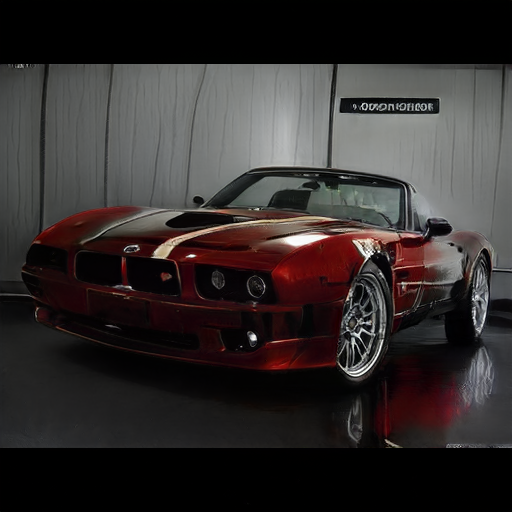
\includegraphics[width=\textwidth]{images/Attempt at reflection.png}
  \caption{Sports convertible}
  \label{fig:reflection}
\end{subfigure}%
\hspace{.02\textwidth}
\begin{subfigure}{.3\textwidth}
  \centering
  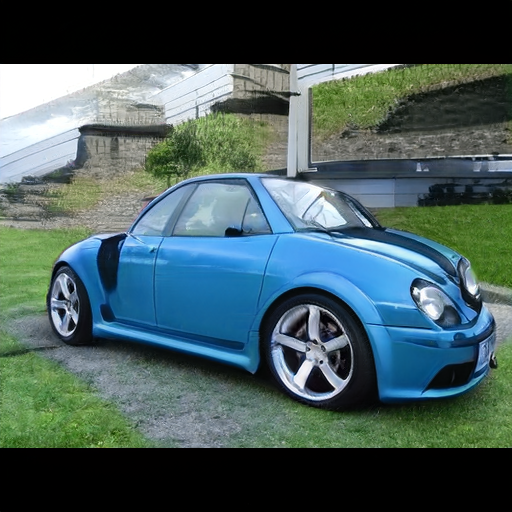
\includegraphics[width=\textwidth]{images/Challenging angle (4).png}
  \caption{Double front car}
  \label{fig:doublefront}
\end{subfigure}
\hspace{.02\textwidth}
\begin{subfigure}{.3\textwidth}
  \centering
  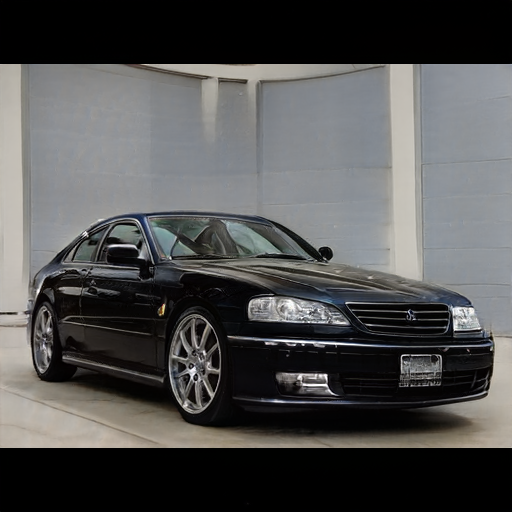
\includegraphics[width=\textwidth]{images/Multi inspired car.png}
  \caption{Multi model inspired design}
  \label{fig:multiinspired}
\end{subfigure}
\captionsetup{width=.85\linewidth}
\caption{Multiple images generated by the used GAN for this project, settings and more info available on the GitHub repository for this project \citep{github_project}.}
\label{fig:straightexports}
\end{figure*}

%------------------------------------
\section{Extending the GANSpace tool}
\label{sec:ganspace_extended}

Since the settled on pre-trained GAN is working as intended, it was also already made to work with the GANSpace tool discussed in the previous assignments \citep{ganspace}.
For this, an extended version of the GANSpace tool was made.
This extended version has a new parameter to specify the used mode should be the one custom made for this project.
Besides this, some features were added to the tool as well, such as an option to export the current canvas, even if it has multiple images on it, all through an easy to use UI.

The extended GANSpace tool works flawlessly once installed, but installation is not as straight forward as it could be.
Since the tool is still relatively unknown and new with available setup instructions missing vital instructions, a more in-depth guide was made available on the GitHub repository for this project \citep{github_project}.
This guide makes use of a fresh install of Ubuntu 20.04 and a system with an NVIDIA GTX970.
Many scripts for and modifications to the GANSpace tool are made to make reproducibility easier.
All of the missing steps not discussed in the original GitHub repository of the GANSpace tool \citep{ganspace_git}, are listed in the thorough documentation of this project's GitHub \citep{github_project}. 


\begin{figure*}
\begin{subfigure}{.45\textwidth}
  \centering
  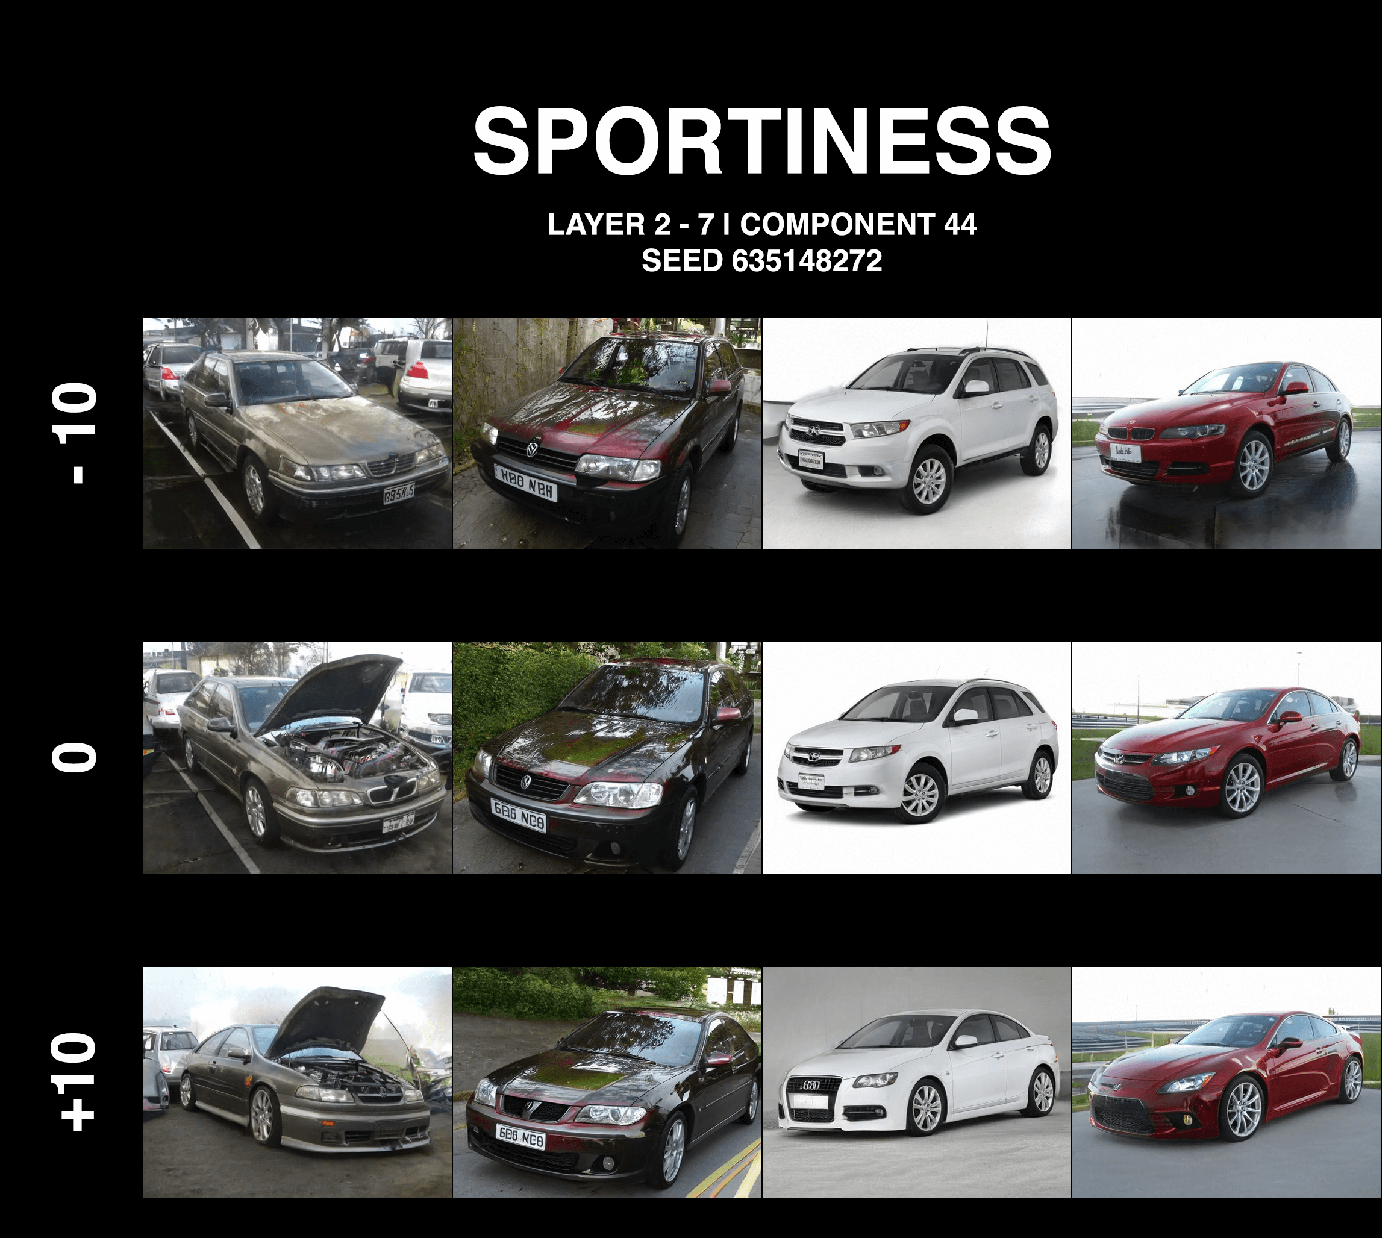
\includegraphics[width=\textwidth]{images/Sportiness.pdf}
  \caption{Component found to influence sportiness of the generated cars.}
  \label{fig:sportiness}
\end{subfigure}%
\hspace{.04\textwidth}
\begin{subfigure}{.45\textwidth}
  \centering
  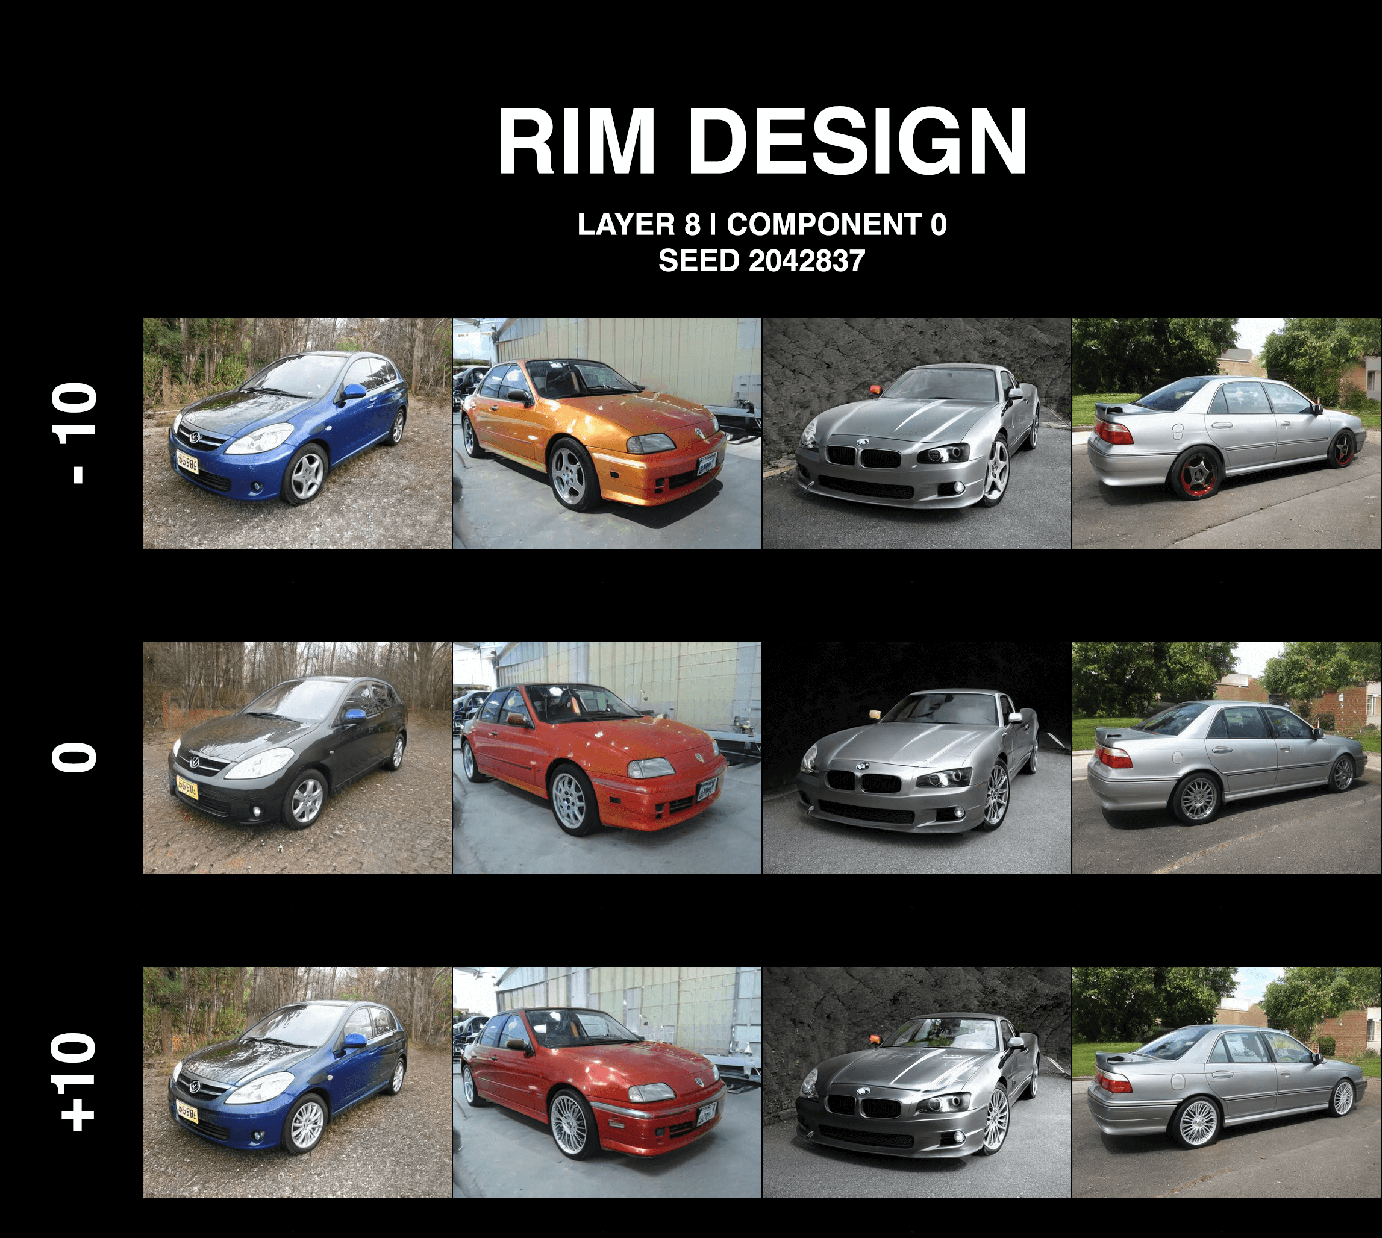
\includegraphics[width=\textwidth]{images/rim_design.pdf}
  \caption{Component found to influence the rim design of the generated cars in a pretty standalone fashion.}
  \label{fig:rimdesign}
\end{subfigure}
\centering
\captionsetup{width=.85\linewidth}
\caption{Baseline images, labeled '0', from the GAN and variants by manipulating interesting found components using the extended GANSpace tool. Settings and more info available on this project's GitHub repository \citep{github_project}.}
\label{fig:ganspaceexports}
\end{figure*}
\part{Evaluation}
\label{part:evaluation}


%------------------------------------
\section{Internal evaluation of the GAN}
\label{sec:internal_validation}

\begin{wrapfigure}{r}{0.4\textwidth}
    \centering
    \vspace*{-20pt}
    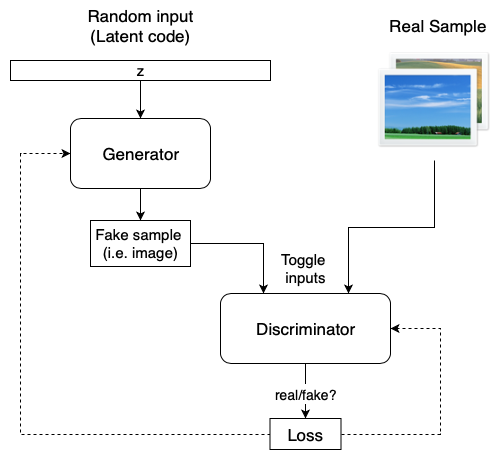
\includegraphics[width=0.35\textwidth]{images/howganwork.png}
    \captionsetup{justification=centering}
    \caption{Illustration on how a GAN works by \citet{how_gan_works}.}
    \label{fig:howganworks}
\end{wrapfigure}

Validation is already a crucial component in the working of a GAN.
A GAN works by training 2 individual AIs, a generator and a discriminator.
The former generates images from scratch.
The discriminator then tries to validate whether the image generated by the generator is real or not.
The training images are thus for the learning algorithm of the discriminator.
The output of the discriminator is then used as a way of validating and evaluating the output of the generator and training it further.
It is clear this process forms a sort of cat and mouse game between both AIs, an analogy often made when talking about GANs.
A visual of this is given in figure \ref{fig:howganworks}, taken from an easy explanation on how StyleGAN works by \citet{how_gan_works}.

So in a way, a GAN is internally evaluated by design.
ProGAN, in many ways a precursor to StyleGAN, also from NVIDIA, was exceptional in the way it works by having a discriminator and generator whose performance increases over time.
This happens by incrementally increasing the resolution, expressed in the number of pixels, of both models.
This idea is still in place with StyleGAN, which again proves a form of internal, increasingly harder, evaluation plays a key role in its working.

%------------------------------------
\section{Building the external evaluation tool}
\label{sec:evaluation_tool}

Since internal evaluation is already taken care of by design, the focus of this project lies in external evaluation.
Besides using the criteria and framework seen in the course, a survey with juries will also be held.
For this survey, a custom PHP tool was developed by modifying a tool used in a previous paper \citep{bapproef} of mine.
A screenshot of the tool is given in figure \ref{fig:eval_tool}.
The flow of this custom made tool is as follows:
\begin{itemize}
    \item Explain what data of the participant will be stored and made available to the public.
    \item Show a short video explaining the different criteria the participant will have to fill out for each image.
    \item Ask personal info about participant:
    \begin{itemize}
        \item Gender, since some car designs might appeal more to a certain gender.
        \item Age group, separated in 5-year intervals to further anomalies the participant info. 
        \item Whether or not the participant has expertise in the domain. A participant is considered to have expertise in the domain if he can recognize cars from different brands from any angle, albeit since he is a passionate car lover or works in a garage or anything in between.
        \item Whether or not the participant is colour blind or has restricted vision during the survey.
    \end{itemize}
    \item Show some 'test images' first that can be used to tackle burn-in of the rating system.
    \item Show images one by one in random order and ask the participant the following using a likert scale from zero to five:
    \begin{itemize}
        \item Quality: an image is considered of good quality if it doesn't contain graphical glitches or artefacts as explained in the introductory video.
        \item Colors: colours of an image are considered good if they are viable in real life. Remember, some colour combinations may be ugly to the participant but still realistic. An image has bad colours if it has purple grass, red shadows...
        \item Creativity: whether the participant finds the image creative is a subjective manner, if the participant recognize (elements of) existing cars (s)he can discuss this in the notes field.
        \item General impression: an overall rating on how pleased the participant is with this car design. This is again subjective with possible further discussion in the notes.
        \item Notes: this field can be used to discuss recognised cars, the reasoning for exceptionally low or high scores and more.
    \end{itemize}
\end{itemize}

%------------------------------------
\section{Further notes on evaluation}
\label{sec:notes_evaluation}

The evaluation criteria are still open for debate.
Initially, the user is told he will see images of both human-made car design through Adobe Photoshop and computer-generated car design.
Whether or not the user is shown an image as human-made or machine-generated is at random and stored in the database.
This was done to combat bias but is again still open for changes.
The tool is already published online \footnote{\url{https://car-design-survey.lennertbontinck.com/}} for feedback purposes of this assignment. 
Note that the introductory video explaining the tool is not yet made and thus not yet available. 

\begin{figure}[H]
    \centering
    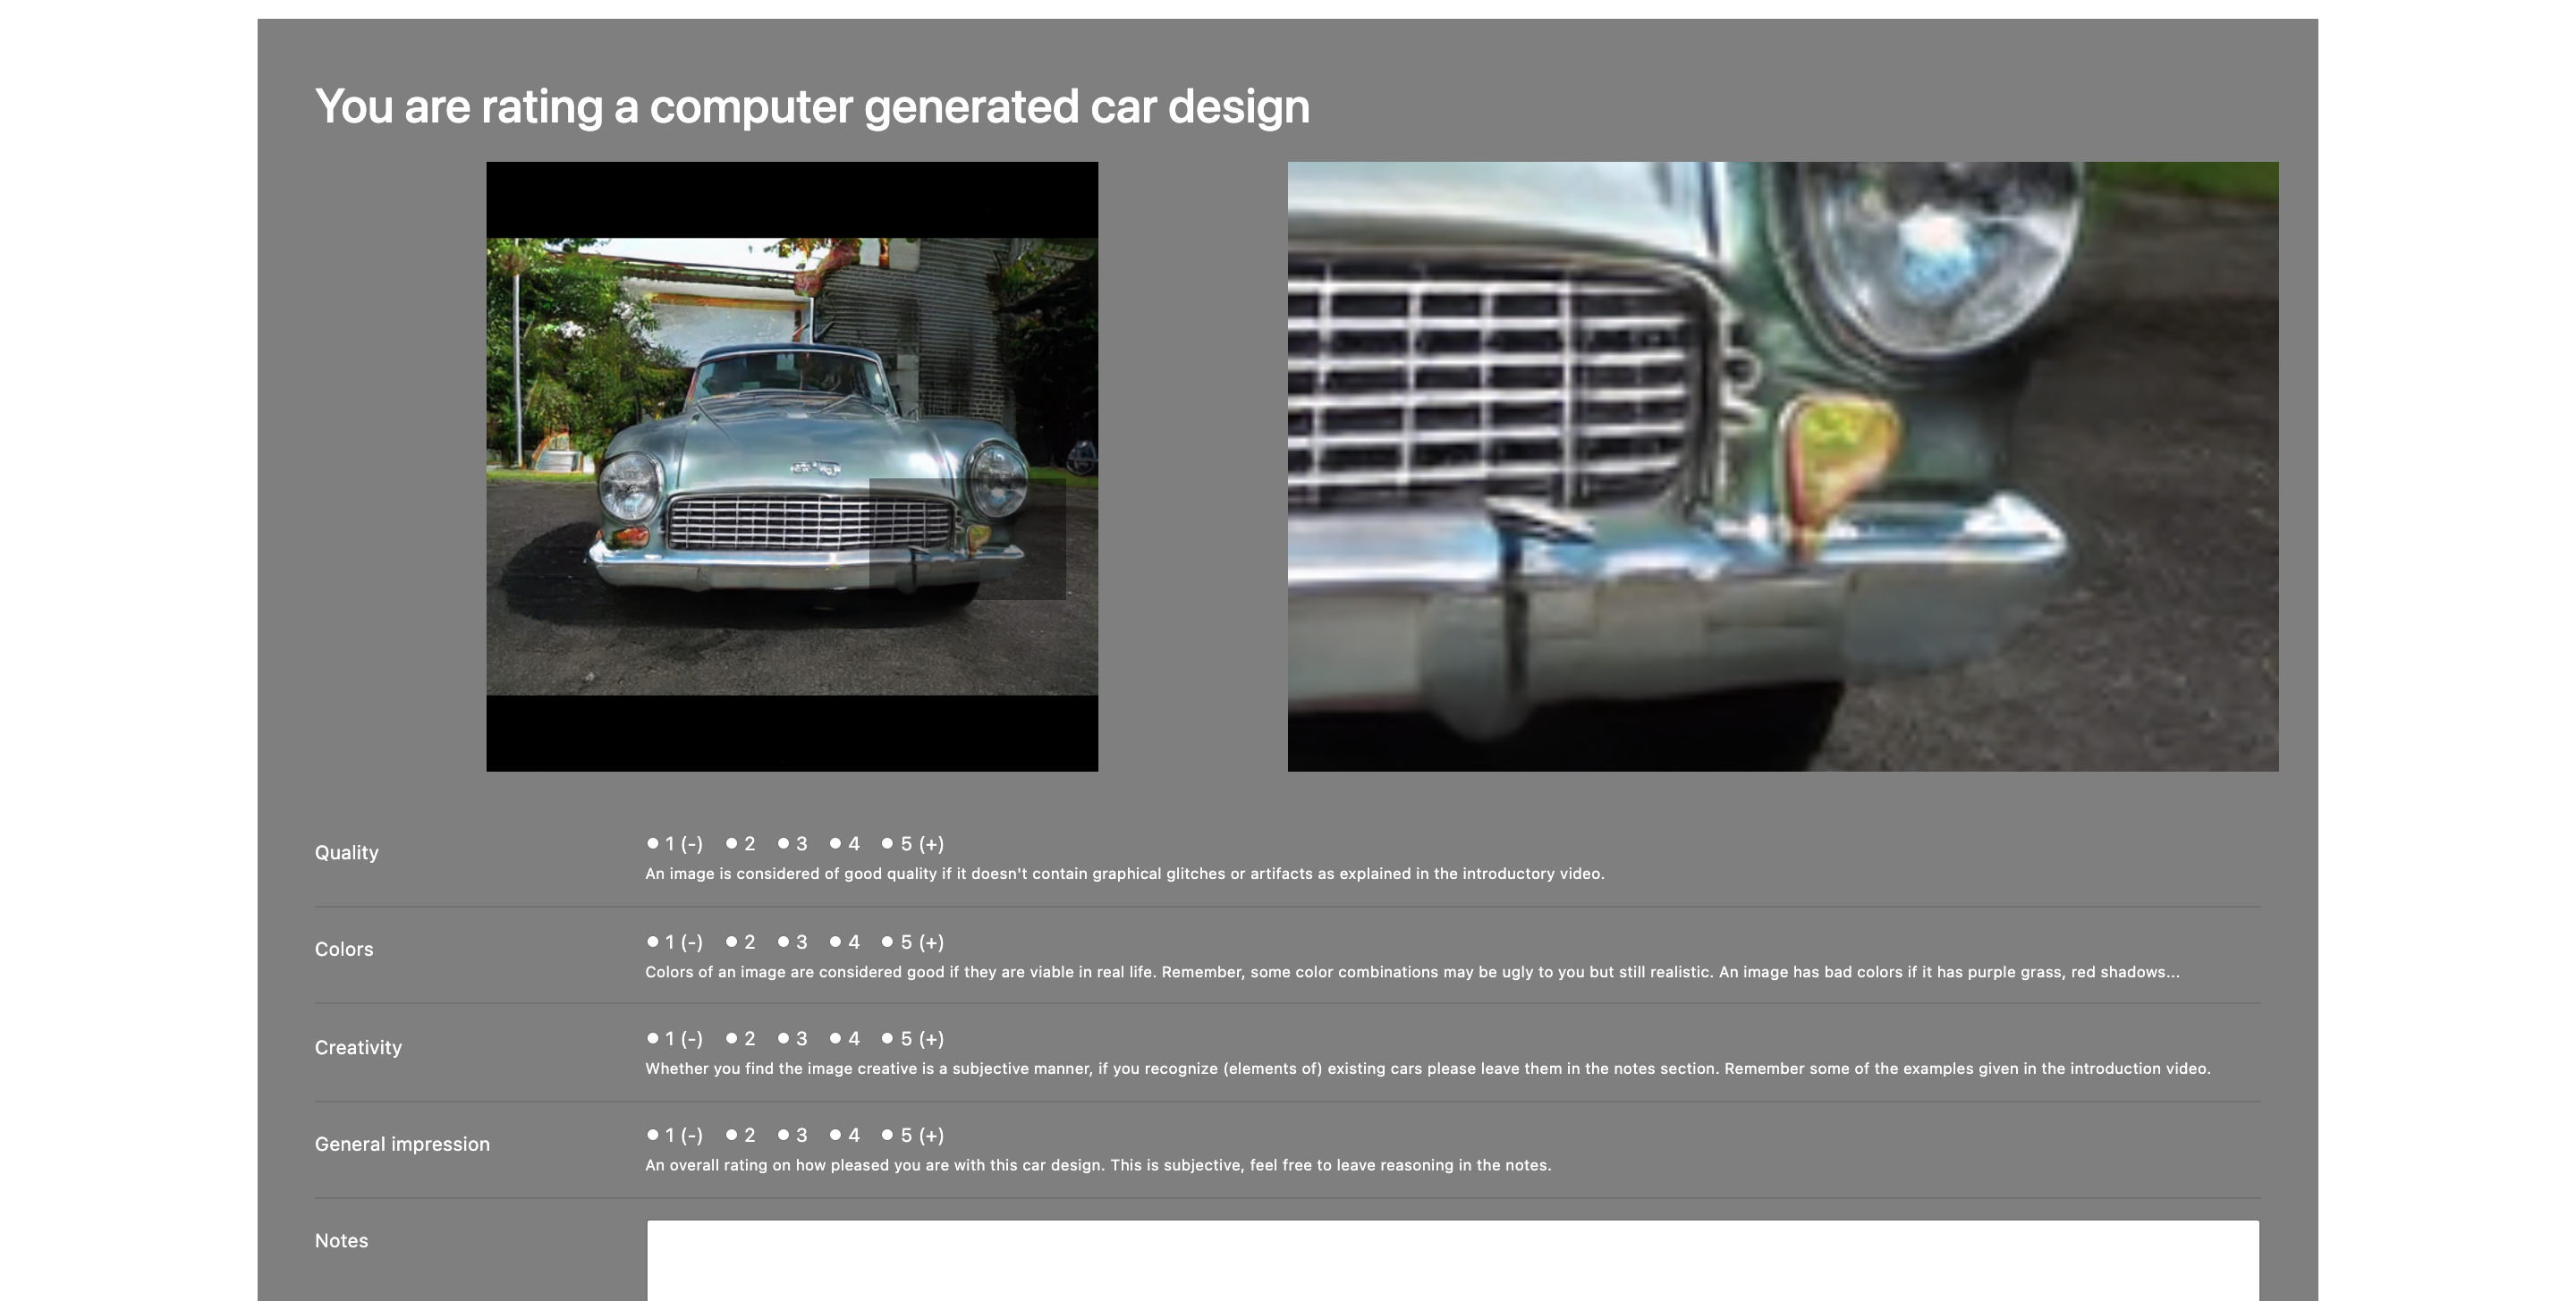
\includegraphics[width=0.85\linewidth]{images/online_survey.png}
    \captionsetup{width=0.85\linewidth}
    \captionsetup{justification=centering}
    \caption{Screenshot of the custom made online survey tool.}
    \label{fig:eval_tool}
\end{figure}
\part{Conclusions}
\label{part:conclusions}
% wat geleerd en wat onduidelijk

%------------------------------------
\section{What has been achieved so far}
\label{sec:issues}

During this assignment, much more than just the evaluation strategy was thought of.
It has been decided what pre-trained GAN will be used and it is working on a fresh Ubuntu install specifically for this project.
the GANSpace tool for control over the GAN is also already installed and even extended after some initial setup difficulties.
A lot of documentation on the setup and use of this tool has also been made on the GitHub repository for this project \citep{github_project}. 
Many interesting images from the GAN and some interesting components found using GANSpace have also already been found and documented on GitHub.

An easy to use, custom made, evaluation tool was also already created.
The tool has already been tested to work online and besides for some small remaining questions, the evaluating process can start soon.
All of this combined with the knowledge from the previous assignments means the road to the final assignment is clear and do-able.


%------------------------------------
\section{Expected roadmap}
\label{sec:roadmap}

Due to the huge progress made in this assignment, the expected roadmap introduced in the previous assignment could be shortened but remains unchanged just in case.
\begin{itemize}
    \item 02/04 - 11/04: Development of the GAN.
    \item 11/04 - 15/04: Control over the GAN and collection of images/videos for evaluation.
    \item 15/04 - 29/04: Collection of evaluation data.
    \item 29/04 - 18/05: Writing of the research paper.
\end{itemize}

%references list
\nocite{*}
\printbibliography[heading=bibintoc, title={References}]
\end{document}
